%%%%
%% thesis.tex
%%
%% Copyright 2010 Jeffrey Finkelstein
%%
%% Except where otherwise noted, this work is made available under the terms of
%% the Creative Commons Attribution-ShareAlike 3.0 license,
%% http://creativecommons.org/licenses/by-sa/3.0/.
%%
%% You are free:
%%    * to Share — to copy, distribute and transmit the work
%%    * to Remix — to adapt the work
%% Under the following conditions:
%%    * Attribution — You must attribute the work in the manner specified by
%%    the author or licensor (but not in any way that suggests that they
%%    endorse you or your use of the work).
%%    * Share Alike — If you alter, transform, or build upon this work, you may
%%    distribute the resulting work only under the same, similar or a 
%%    compatible license.
%%    * For any reuse or distribution, you must make clear to others the 
%%    license terms of this work. The best way to do this is with a link to the
%%    web page http://creativecommons.org/licenses/by-sa/3.0/.
%%    * Any of the above conditions can be waived if you get permission from
%%    the copyright holder.
%%    * Nothing in this license impairs or restricts the author's moral rights.
%%%%
\documentclass[draft]{article}
%\documentclass{article}

% package imports
\usepackage[noend,linesnumbered,boxed]{algorithm2e} % for creating pseudocode
\usepackage{amsmath} % for piecewise function definition
\usepackage{amsthm} % for theorems, definitions, lemmas, and styles
\usepackage{amssymb} % for strict subset symbol (\subsetneq)
\usepackage{chngcntr} % for counting figures with section numbers
\usepackage{complexity} % for typesetting complexity classes
\usepackage{cclicenses} % for adding creative commons license symbols
\usepackage[margin=1in]{geometry} % for setting page margins
\usepackage{graphicx} % for including images
\usepackage[pdftitle={On computational complexity of equivalence relations},
  pdfauthor={Jeffrey Finkelstein}]{hyperref}
\usepackage[all]{hypcap} % references to images will link to the image
\usepackage{multicol} % for list split over multiple columns

% don't print semicolons in pseudocode algorithms
\dontprintsemicolon

% define theorem, lemma, and definition environments and corresponding styles
\newtheorem{theorem}{Theorem}%[section]
\newtheorem{lemma}{Lemma}%[section]
\newtheorem{corollary}{Corollary}%[section]
\theoremstyle{definition} 
\newtheorem{definition}{Definition}%[section]

% define lemma, corollary, and definition context labels for /autoref command
\newcommand{\lemmaname}{Lemma}
\newcommand{\corollaryname}{Corollary}
\newcommand{\definitionname}{Definition}

% custom shortcut commands
\newcommand{\plain}[1]{\,\text{#1}\,} % plain text inside math environments
\newcommand{\sigmastar}{\Sigma^{*}}
\newcommand{\kr}{\leq^{p}_{ker}} % kernel-reduces
\newcommand{\nkr}{\nleq^{p}_{ker}} % does not kernel-reduce
\newcommand{\kequiv}{\equiv^{p}_{ker}} % is equivalent under kernel reductions
\newcommand{\mor}{\leq^{p}_{m}} % many-one reduces
\newcommand{\moequiv}{\equiv^{p}_m} % is equivalent under many-one reductions
\newcommand{\tequiv}{\equiv^{p}_T} % is equivalent under Turing reductions

% create the creative commons license
\newcommand{\license}{\begin{tabular}[h]{r l}
    \bysa & \parbox{275pt}{Copyright 2010 Jeffrey Finkelstein. 
      Except where otherwise noted, this work is licensed
      under http://creativecommons.org/licenses/by-sa/3.0/}
\end{tabular}}

% set commands for \ACCEPT and \REJECT for use in algorithms
\SetKw{ACCEPT}{accept}
\SetKw{REJECT}{reject}

% redefine footnote so it has no reference and no number
\long\def\symbolfootnote#1{\begingroup%
\def\thefootnote{\fnsymbol{footnote}}\footnotetext{#1}\endgroup} 

% change figure numbering so it is per section
%\counterwithin{figure}{section}

% define the author, title, and date
\author{Jeffrey Finkelstein} 
\title{On the computational complexity of equivalence relations}
\date{\today} 

\begin{document}
\maketitle
\symbolfootnote{\license}

\begin{abstract}
  In this paper we analyze the notion of kernel reductions among equivalence
  problems, as defined in Fortnow and Grochow, especially with respect to graph
  isomorphism and its polynomial time many-one equivalent problems. We first
  examine some examples of kernel reductions among equivalence problems
  decidable in polynomial time. In doing so, we consider the possibility of
  whether the equality relation is in fact complete under kernel reductions
  with respect to equivalence problems decidable in polynomial time. We then
  examine the complexity of equivalence problems and kernel reductions in
  \NP. We show that most known many-one reductions among isomorphism problems
  in $\NP$ are indeed kernel reductions.
\end{abstract}

\begin{definition}
  Let $R\subseteq\sigmastar\times\sigmastar$. Then $R$ is an \emph{equivalence
    relation} if the following conditions hold:
  \renewcommand{\labelenumi}{\roman{enumi}.}
  \begin{enumerate}
  \item (reflexivity) $\forall x\in\sigmastar$, $(x, x)\in R$
  \item (symmetry) $\forall x,y\in\sigmastar$, if $(x,y)\in R$ then $(y,x)\in
    R$
  \item (transitivity) $\forall x,y,z\in\sigmastar$, if $(x,y)\in R$ and
    $(y,z)\in R$ then $(x,z)\in R$
  \end{enumerate}
  If $(x,y)\in R$, we say \emph{$x$ relates to $y$}, and we write $x\sim y$.
\end{definition}

In \cite{fg09}, Fortnow and Grochow give a formal definition of a new class of
languages: the class of equivalence problems which can be decided in polynomial
time. They also provide a natural reduction for this class of problems. We
provide the definitions, along with their generalizations in \NP, here.

\begin{definition}\label{def:peq}
  \textit{\PEq} is the class of equivalence relations whose membership can be
  decided in polynomial time.

  \textit{\NPEq} is the class of equivalence relations whose membership can be
  decided in nondeterministic polynomial time.
\end{definition}

\begin{definition}\label{def:kr}
  Let $R$ and $S$ be equivalence relations. We say $R$ \textit{polynomial time
  kernel reduces to} $S$ if $\exists f\in\FP:\forall x,y\in\sigmastar (x, y)\in
  R \iff (f(x),f(y))\in S$. We denote this by $R\kr S$.
  
  We say $R$ \textit{is kernel equivalent to} $S$ if $R\kr S$ and $S\kr R$. We
  denote this by $R\kequiv S$.
\end{definition}

Note the difference between a kernel reduction and a many-one reduction: a
kernel reduction maps $(x,y)\in R$ to $(f(x), f(y))\in S$, whereas a many-one
reduction maps $(x,y)\in R$ to $f(x, y)\in S$, for some polynomial time
computable function $f$. Informally, a many-one reduction gets access to both
$x$ and $y$, but a kernel reduction gets access to only one at a time. Because
the many-one reduction seems to be at least as powerful as the kernel
reduction, we can prove the following lemma.

\begin{lemma}\label{lem:kr_mor}If $A\kr B$ then $A\mor B$.\end{lemma}
\begin{proof}
  Since $A\kr B$, $\exists f\in\FP: (x,y)\in A\iff(f(x), f(y))\in B$. Define
  $g\in FP$ by $g(x,y)=(f(x), f(y))$. Therefore $A\mor B$ by $g$.
\end{proof}

As an analog to polynomial time many-one completeness in \NP, we define a
similar notion of polynomial time completeness under kernel reductions in
\NPEq.

\begin{definition}\label{def:kernel_complete}
  An equivalence relation $R$ is \textit{$\PEq$-complete} if $R\in\PEq$ and
  $\forall S\in\PEq$, $S\kr R$.

  An equivalence relation $R$ is \textit{$\NPEq$-complete} if $R\in\NPEq$ and
  $\forall S\in\NPEq$, $S\kr R$.
\end{definition}

With these definitions in place, we can now define some examples of equivalence
relations in $\PEq$, tractable equivalence problems.

%% TODO should I make a note about assuming |x|=|y|
\begin{definition}
  $R_{par}=\{(x, y)|x$ and $y$ have the same parity$\}$
\end{definition}
\begin{definition}
  $R_{bc}=\{(x, y)|x$ and $y$ have the same number of ones$\}$
\end{definition}
\begin{definition}
  $R_{eq}=\{(x, y)|x=y\}$. This is called the \emph{equality relation}.
\end{definition}
\begin{definition}
  $R_{eqi}=\{(x, y)|x=y$ or $x=\bar{y}\}$
\end{definition}
\begin{definition}
  Let $a\in\sigmastar$. $R_{a}=\{(x,y)|x=y$ or $x\oplus y=a\}$. (Note that
  $R_{a}$ is a family of equivalence relations; $R_{a}$ is a different relation
  for each fixed $a$.)
\end{definition}
%% \begin{definition}
%%   $R_{maj}=\{(x,y)|$ at least half of the bits in both $x$ and $y$ are ones, or
%%   fewer than half of the bits in both $x$ and $y$ are ones$\}$
%% \end{definition}
%% \begin{definition}
%%   Let $k\in\mathbb{N}$. $R_{tk}=\{(x,y)|x$ and $y$ both have at least $k$ ones
%%   or $x$ and $y$ both have fewer than $k$ ones$\}$. (Note that $R_{tk}$ is a
%%   family of equivalence relations; $R_{tk}$ is a different relation for each
%%   fixed $k$. Notice also that if $k=|x|/2$ then $R_{tk}=R_{maj}$.)
%% \end{definition}

Notice the following equivalent definitions, where $n=|x|=|y|=|a|$:
$R_{eq}=\{(x, y)|x \oplus y = 0^n\}$, $R_{eqi}=\{(x, y)|x \oplus y = 0^n$ or
$x\oplus y = 1^n\}$, and $R_{a}=\{(x,y)|x \oplus y = 0^n$ or $x \oplus y\ =
a\}$.

%% TODO show that all the stated equivalence relations are actually eq. rel.s
\begin{theorem}$R_{eq} \subsetneq R_{bc} \subsetneq R_{par}$\end{theorem}
\begin{proof}
  Let $(x, y)\in R_{eq}$, so $x=y$. Then $x$ has exactly the same number of
  ones as $y$ (and the same number of zeros, and in the same order), so $(x, y)
  \in R_{bc}$. Therefore, $R_{eq} \subset R_{bc}$.
 
  Consider $x=1100$ and $y=0101$. Then $(x, y)\in R_{bc}$ but $(x, y) \notin
  R_{eq}$. Therefore $R_{eq} \neq R_{bc}$.

  Let $(x, y)\in R_{bc}$, so $x$ and $y$ have the same number of ones. Let $k$
  be the number of ones in $x$, and $l$ be the number of ones in $y$. Then
  $l=k$, which implies $l \equiv k$ (mod 2). Therefore $x$ and $y$ have
  the same parity, so $(x, y)\in R_{par}$. Therefore $R_{bc} \subset R_{par}$.

  Consider $x=1000$ and $y=1011$. Then $(x, y)\in R_{par}$ but $(x, y) \notin
  R_{bc}$. Therefore $R_{bc} \neq R_{par}$.
\end{proof}

\begin{theorem}$R_{eq} \subsetneq R_{eqi}$\end{theorem}
\begin{proof}
  Let $(x, y)\in R_{eq}$, so $x=y$. Then $(x, y)$ satisfies the property
  specified in the definition of $R_{eqi}$, specifically that $x=y$, so
  $(x, y) \in R_{eqi}$. Therefore $R_{eq} \subset R_{eqi}$.

  Consider $x=1000$ and $y=0111$. Then $(x, y)\in R_{eqi}$ but $(x, y) \notin
  R_{eq}$. Therefore $R_{eq} \neq R_{eqi}$.
\end{proof}

\autoref{fig:containments} exhibits the containments among $R_{eq}$, $R_{eqi}$,
$R_{bc}$, and $R_{par}$. Note that if $a=0^n$, for $n=|x|=|y|$, then
$R_{a}=R_{eq}$ and if $a=1^n$ then $R_{a}=R_{eqi}$.

\begin{figure}
  \begin{center}
    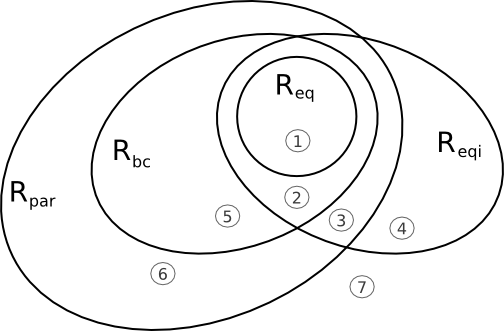
\includegraphics[width=300pt,height=241pt,keepaspectratio=true]
                    {containments.png}
  \end{center}
  \caption{ \label{fig:containments} Containment relationships for equivalence
    relations $R_{eq}$, $R_{eqi}$, $R_{bc}$, and $R_{par}$. The following are
    example elements in the sets at the specified locations: 1. (1100, 1100)
    2. (1010, 0101) 3. (1000, 0111) 4. (10000, 01111) 5. (1000, 0001) 6. (1000,
    1011) 7. (1000, 0000) }
\end{figure}

Since membership in $R_{par}$, $R_{bc}$, $R_{eq}$, $R_{eqi}$, and $R_a$ can be
decided in polynomial time, they are all members of \PEq. Now we can examine
kernel reductions between these members of \PEq. Notice that the following
reductions reduce the more general equivalence relation to the more restrictive
equivalence relation.

\begin{theorem}$R_{par}\kr R_{bc}$\end{theorem}
\begin{proof}
  Construct $M\in \FP$ on input $w\in\sigmastar$:\\
  \begin{algorithm}[H]
    \For{$i=1$ \KwTo $|w|-1$}{
      \If{$w_i=1$}{
        \For{$j=i+1$ \KwTo $|w|$}{
          \If{$w_j=1$}{
            write 0 to both $w_i$ and $w_j$\;
            break\;
          }
        }
      }
    }
  \end{algorithm}
  Notice that this is the machine which finds pairs of ones and writes zeros in
  their place, one pair at a time.

  Suppose $(x, y)\in R_{par}$, so either $x$ and $y$ both have even parity or
  $x$ and $y$ both have odd parity.
  
  If $x$ and $y$ both have even parity, $x$ contains $2k$ ones and $y$ contains
  $2l$ ones, for some $k,l\in\mathbb{N}$. $M(x)$ and $M(y)$ both output the
  string $0^{|x|}$, and since both $M(x)$ and $M(y)$ have a bitcount of zero,
  $(M(x), M(y))\in R_{bc}$.

  If $x$ and $y$ both have odd parity, $x$ contains $2k+1$ ones and $y$
  contains $2l+1$ ones, for some $k,l\in\mathbb{N}$. $M(x)$ and $M(y)$ both
  output a string containing a single one, so both $M(x)$ and $M(y)$ have a
  bitcount of one, $(M(x), M(y))\in R_{bc}$.

  Suppose $(x, y)\notin R_{par}$, so without loss of generality, $x$ has even
  parity and $y$ has odd parity. Then $x$ contains $2k$ ones and $y$ contains
  $2l+1$ ones, for some $k,l\in\mathbb{N}$. Thus $M(x)$ outputs the string
  $0^{|x|}$ and $M(y)$ outputs the string containing a single one. Since the
  bitcount of $M(x)$ is zero and the bitcount of $M(y)$ is one,
  $(M(x), M(y))\notin R_{bc}$.

  Therefore $(x, y)\in R_{par} \iff (M(x), M(y))\in R_{bc}$, so
  $R_{par} \kr R_{bc}$.
\end{proof}

\begin{theorem}$R_{bc}\kr R_{eq}$\end{theorem}
\begin{proof}
  Construct $M\in \FP$ on input $w\in\sigmastar$ which sorts the bits of $w$
  using an efficient (polynomial-time) sorting algorithm. Notice that if
  $|w|=n$ and $w$ contains $k$ ones, this machine outputs the string
  $0^{n-k}1^k$.

  Suppose $(x, y)\in R_{bc}$, so $x$ and $y$ have the same number of ones, say
  $k$. Thus $M(x)=M(y)=0^{n-k}1^k$, so $(M(x), M(y))\in R_{eq}$.
  
  Suppose $(x, y)\notin R_{bc}$, so $x$ and $y$ have a different number of
  ones. Suppose $x$ has $k$ ones and $y$ has $l$ ones, for some
  $k,l\in\mathbb{N}$. Assume without loss of generality that $k>l$. Then
  $M(x)=0^{n-k}1^{k}$ and $M(y)=0^{n-l}1^{l}$, so $M(x)\neq M(y)$. Thus
  $(M(x), M(y))\notin R_{eq}$.

  Therefore $(x, y)\in R_{bc} \iff (M(x), M(y))\in R_{eq}$, so $R_{bc}\kr
  R_{eq}$.
\end{proof}

\begin{theorem}\label{thm:reqi_req}$R_{eqi}\kr R_{eq}$\end{theorem}
\begin{proof}
  Construct machine $M\in\FP$ on input $w\in\sigmastar$, where
  $w=w_1w_2\cdots w_{|w|}$:\\
  \begin{algorithm}[H]
    \eIf{$w_1=0$}{
      \Return{$w$}
    }{
      \Return{$\bar{w}$}
    }
  \end{algorithm}
  
  Suppose $(x,y)\in R_{eqi}$, so either $x=y$ or $x=\bar{y}$. In the case that
  $x=y$, $M(x)$ and $M(y)$ produce the same output. In the case that
  $x=\bar{y}$, then either $x_1=1$ and $y_1=0$ or $x_1=0$ and $y_1=1$. Consider
  without loss of generality the case that $x_1=1$ and $y_1=0$. Then $M(x)$
  outputs $\bar{x}$ and $M(y)$ outputs $y$. Now $\bar{x}=\bar{\bar{y}}=y$, so
  $M(x)=M(y)$. Therefore $(M(x),M(y))\in R_{eq}$.

  Suppose $(x,y)\notin R_{eqi}$, so $x\neq y$ and $x\neq\bar{y}$. In the case
  that $x_1=0$ and $y_1=0$, then $M(x)=x$ and $M(y)=y$. Since $x\neq y$, then
  $M(x)\neq M(y)$, so $(M(x),M(y))\notin R_{eq}$. In the case that $x_1=0$ and
  $y_1=1$, then $M(x)=x$ and $M(y)=\bar{y}$. Since $x\neq\bar{y}$, then
  $M(x)\neq M(y)$, so $(M(x),M(y))\notin R_{eq}$. In the case that $x_1=1$ and
  $y_1=0$, then $M(x)=\bar{x}$ and $M(y)=y$. Since $x\neq\bar{y}$, then
  $\bar{x}\neq \bar{\bar{y}}=y$, so $M(x)\neq M(y)$, and $(M(x),M(y))\notin
  R_{eq}$. In the case that $x_1=1$ and $y_1=1$, then $M(x)=\bar{x}$ and
  $M(y)=\bar{y}$. Since $x\neq y$, then $\bar{x}\neq\bar{y}$, so $M(x)\neq
  M(y)$, and $(M(x),M(y))\notin R_{eq}$.

  Therefore $(x,y)\in R_{eqi}\iff (M(x), M(y))\in R_{eq}$, so $R_{eqi}\kr
  R_{eq}$.
\end{proof}

\begin{theorem}Let $a\in\sigmastar$. Then $R_a\kr R_{eq}$.\end{theorem}
\begin{proof}
  Construct machine $M\in\FP$ on input $w\in\sigmastar$, where $|w|=|a|=n$,
  $w=w_1w_2\cdots w_n$ and $a=a_1a_2\cdots a_n$:\\
  \begin{algorithm}[H]
    $s\gets((a_1, w_1), (a_2, w_2), \ldots, (a_n, w_n))$\;
    Perform a stable sort on $s$ with each $a_i$ as the key, to obtain two
    subsequences, $r$ and $r'$, where $r=(a_i, w_i)|_{a_i=0}$ and $r'=(a_j,
    w_j)|_{a_j=0}$\;
    Run the algorithm in \autoref{thm:reqi_req} on the concatenation of each
    $w_j$ in $r'$ to obtain a new string $c$\;
    \Return{the concatenation of each $w_i$, in the order of $r$, with the
      string $c$}
  \end{algorithm}
  Notice that informally this machine splits up the problem into two easier
  problems whose solutions are known: the first problem is the problem of
  determining equality, the second problem is the problem of determining either
  equality or bitwise complement.

  Suppose $(x,y)\in R_a$, so either $x=y$ or $x\oplus y=a$. In the case that
  $x=y$, then $M(x)$ and $M(y)$ output the same string, so $M(x)=M(y)$, and
  hence $(M(x),M(y))\in R_{eq}$. Now consider the case in which $x\oplus y=a$,
  which implies $x\oplus a=y$ and $y\oplus a=x$. Then $M(x)$ and $M(y)$ will
  first rearrange the bits of $x$ and $y$, respectively, by stable sorting the
  bits of $a$. For all bits of $a$ which are zero, the corresponding bits of
  $x$ and $y$ are equal, by hypothesis. For all bits of $a$ which are one, the
  corresponding bits of $x$ and $y$ are complements of one another. Let $a_i$
  be the leftmost bit of $a$ which is one. In the case that $x_i=1$ and
  $y_i=0$, then the algorithm from \autoref{thm:reqi_req} will flip all the
  bits of $x$ corresponding to bits of $a$ which are one. Since $y$ and $x$
  were complements, at these bits only, now $M(x)=M(y)$, so $(M(x),M(y))\in
  R_{eq}$. The argument for the case that $x_i=0$ and $y_i=1$ is symmetric.

  Suppose $(x,y)\notin R_a$, so $x\neq y$ and $x\oplus y\neq a$. So $\exists
  i,j\in\{1,2,\ldots,|x|\}: x_i\neq y_i$ and $x_j\oplus y_j\neq a$. Now $M(x)$
  and $M(y)$ will rearrange the bits of $x$ and $y$, respectively, by stable
  sorting the bits of $a$. Call these new strings $x'$ and $y'$, and the
  corresponding permutation of indices $i$ and $j$, $i'$ and $j'$,
  respectively. If $a_{i'}$ is zero then $x_{i'}\neq y_{i'}$.

  %% TODO complete this proof
\end{proof}

It seems that all of these ``bitwise'' equivalence problems reduce to the
equality relation, $R_{eq}$, which seems to be the most restrictive equivalence
relation in \P. Indeed, there are as many equivalence classes as there are
unique strings, because each string is its own equivalence class. Is the
equality relation \PEq-complete? To provide more evidence We will next examine
an equivalence problem in \P that is not explicitly a problem involving the
examination of bits in a string.

\begin{definition}
  Let $T_1=(V_1, E_1, r_1), T_2=(V_2, E_2, r_2)$, with $r_1\in V_1$ and $r_2\in
  V_2$, be rooted trees. Then $T_1$ is \emph{isomorphic to} $T_2$ if
  $\exists\phi:V_1\to V_2:\phi(r_1)=r_2$ and $(u,v)\in E_1\iff(\phi(u),
  \phi(v))\in E_2$.
\end{definition}
\begin{definition}
  $TI=\{(T_1,T_2)|T_1$ is isomorphic to $T_2\}$
\end{definition}
Informally, two trees are isomorphic if there is a permutation of the vertices
of one tree which preserves edges in the other tree and preserves the root
node.

The tree isomorphism problem is in $\P$, and in fact, easier than \P. For a
linear time algorithm for deciding isomorphism of trees see \cite{ahu74}, and
for an alternating logarithmic time algorithm see \cite{buss97}.

%% TODO tree canonization is in CF(FALOGTIME)\subset CF(P)
%% TODO do the tree isomorphism algorithms reduce to equality?

If the equality relation is \PEq-complete, then some collapses happen, as
described in \cite{fg09}. We first restate the definition of another complexity
class defined in \cite{fg09} (defined there as $\KerFP$).

\begin{definition}
  Let $R$ be an equivalence relation, an let $f\in\FP$. Then $f$ is a
  \emph{complete invariant} for $R$ if $(x,y)\in R$ if and only if $f(x)=f(y)$.
\end{definition}
\begin{definition}
  $\FPKer=\{L|L$ is an equivalence relation with a complete invariant in
  $\FP\}$
\end{definition}

\begin{lemma}\label{lem:ker_peq}
  $\FPKer\subseteq\PEq$
\end{lemma}
\begin{proof}
  Let $R\in\FPKer$. Then by definition $\exists f\in\FP: (x,y)\in R\iff
  f(x)=f(y)$. To decide membership of $(x,y)\in\R$, use $f$ to decide whether
  $f(x)=f(y)$. This is true if and only if $(x,y)\in R$. Therefore membership
  in $R$ can be decided in polynomial time, hence $\FPKer\subseteq\PEq$.
\end{proof}

For the sake of clarity, we provide a proof of the following claim made by
Fortnow and Grochow:

\begin{theorem}
  $\FPKer=\PEq$ if and only if $R_{eq}$ is \PEq-complete.
\end{theorem}
\begin{proof}
  For the forward direction, suppose $\FPKer=\PEq$. Let $S\in\PEq=\FPKer$, so
  $\exists f\in\FP: (x,y)\in S\iff f(x)=f(y)\iff (f(x),f(y))\in R_{eq}\iff S\kr
  R_{eq}$. Thus $R_{eq}$ is \PEq-complete.

  Conversely, suppose $R_{eq}$ is \PEq-complete. Then $\forall S\in\PEq$,
  $\exists f\in\FP:(x,y)\in S\iff(f(x),f(y))\in R_{eq}\iff f(x)=f(y)$. Thus $f$
  is a complete invariant for $S$ computable in polynomial time. Thus
  $S\in\FPKer$, and hence $\PEq\subseteq\FPKer$. By \autoref{lem:ker_peq},
  $\FPKer\subseteq\PEq$, therefore $\PEq=\FPKer$.
\end{proof}

Fortnow and Grochow provide evidence that $R_{eq}$ is \emph{not} \PEq-complete,
by showing that something crazy happens if $\FPKer=\PEq$. Specifically, if
$\FPKer=\PEq$ then $\UP\subseteq\BQP$\cite{fg09}.

%% TODO restate FG09 Thm 4.3 If Ker=PEq then UP\subseteq BQP,  Cor 4.8 (pf?)
%% note: this is apparently evidence that PEq is not equal to Ker

%% TODO showing completeness of a problem should be somewhat easier because we
%% are allowed to examine the entire computation history

%% TODO start a new section here

An equivalence problem of particular importance is the graph isomorphism
problem. Although it is in \NP, it is not known to be \NP-complete and it is
not known to be in \P. It is therefore a candidate for $\NP\backslash\P$ (if
$\P\neq\NP$). Since it is an equivalence problem in \NP, it is a member of
\NPEq, so it may be of particular value to study kernel reductions to and from
the graph isomorphism problem. We begin by examining kernel reductions from the
$\PEq$ equivalence relations defined above to the graph isomorphism problem.
The reductions should intuitively be easy because the graph isomorphism problem
is (seemingly) of greater complexity.

\begin{definition}
  $GI=\{(G_1, G_2)|G_1$ and $G_2$ are undirected graphs and $G_1$ is isomorphic
  to $G_2\}$
\end{definition}

\begin{theorem}\label{thm:rpar_gi}$R_{par}\kr GI$\end{theorem}
\begin{proof}
  Construct $M\in \FP$ on input $w\in\sigmastar$:\\
  \begin{algorithm}[H]
    $V_w\gets\{v_p, v_o\}$\;
    $E_w\gets\{\}$ \tcp{undirected edges}\;
    \For{$i=1$ \KwTo $|w|$}{
      \If{$w_i=1$}{
        \eIf{$(v_o, v_p)\in E_w$}{add undirected edge $(v_o, v_p)$ to $E_w$\;}
            {remove $(v_o, v_p)$ from $E_w$\;}
      }
    }
    \Return $G_w=(V_w, E_w)$
  \end{algorithm}

  Suppose $(x, y)\in R_{par}$, so either $x$ and $y$ both have even parity or
  $x$ and $y$ both have odd parity. 

  If $x$ and $y$ both have even parity, $x$ contains $2k$ ones and $y$ contains
  $2l$ ones, for some $k,l\in\mathbb{N}$. Since $2k$ is even, machine $M$ on
  input $x$ adds then removes the edge $(v_o, v_p)$ to and from $E_x$ an equal
  number of times. Similarly for $M$ on input $y$. Therefore $M(x)$ outputs
  $G_x=(V_x, E_x)$, where $V_x=\{v_o, v_p\}$ and $E_x=\{\}$, and $M(y)$ outputs
  $G_y=(V_y, E_y)$, where $V_y=\{v_o, v_p\}$ and $E_y=\{\}$. Then $G_x$ is
  isomorphic to $G_y$ by the identity function, $I:V_x\to V_y$, defined by
  $I(v)=v, \forall v\in V_x$.

  If $x$ and $y$ both have odd parity, $x$ contains $2k+1$ ones and $y$
  contains $2l+1$ ones, for some $k,l\in\mathbb{N}$. Since $2k+1$ is odd,
  machine $M$ on input $x$ adds edge $(v_o, v_p)$ to $E_x$ one more time than
  it removes the edge. Similarly for $M$ on input $y$. Therefore $M(x)$ outputs
  $G_x=(V_x, E_x)$, where $V_x=\{v_o, v_p\}$ and $E_x=\{(v_o, v_p)\}$, and
  $M(y)$ outputs $G_y=(V_y, E_y)$, where $V_y=\{v_o, v_p\}$ and $E_y=\{(v_o,
  v_p)\}$. Then $G_x$ is isomorphic to $G_y$ by the identity function,
  $I:V_x\to V_y$, defined by $I(v)=v, \forall v\in V_x$.

  Suppose $(x, y)\notin R_{par}$, so without loss of generality, $x$ has even
  parity and $y$ has odd parity. Then $x$ contains $2k$ ones and $y$ contains
  $2l+1$ ones, for some $k,l\in\mathbb{N}$. Since $2k$ is even, machine $M$ on
  input $x$ adds then removes the edge $(v_o, v_p)$ to and from $E_x$ an equal
  number of times. Since $2l+1$ is odd, machine $M$ on input $y$ adds edge
  $(v_o, v_p)$ to $E_y$ one more time than it removes the edge. Therefore
  $M(x)$ outputs $G_x=(V_x, E_x)$, where $V_x=\{v_o, v_p\}$ and $E_x=\{\}$, and
  $M(y)$ outputs $G_y=(V_y, E_y)$, where $V_y=\{v_o, v_p\}$ and $E_y=\{(v_o,
  v_p)\}$. Since $(v_o, v_p)\in E_y$ but $(v_o, v_p)\notin E_x$, so no
  bijection exists between $V_x$ and $V_y$ which preserves edges. Therefore,
  $G_x$ is not isomorphic to $G_y$ so $(M(x), M(y))\notin GI$.

  Therefore $(x, y)\in R_{par} \iff (M(x), M(y)) \in GI$, so $R_{par} \kr GI$.
\end{proof}

\begin{theorem}\label{thm:rbc_gi}$R_{bc}\kr GI$\end{theorem}
\begin{proof}
  Construct $M\in \FP$ on input $w \in \sigmastar$:\\
  \begin{algorithm}[H]
    $V_w\gets\{v_1, v_2, \ldots, v_{|w|}, v_{zero}, v_{one,0}, v_{one,1},
    v_{one,2}\}$\;
    $E_w\gets\{(v_{one,0}, v_{one,1}), (v_{one,1}, v_{one,2}), (v_{one,2},
    v_{one,0})\}$\tcp{undirected edges}\; 
    \For{$i=1$ \KwTo $|w|$}{
      \eIf{$w_i=1$}{
        add undirected edge $(v_i, v_{one,0})$ to $E_w$\;
      }{
        add undirected edge $(v_i, v_{zero})$ to $E_w$\;
      }
    }
    \Return{$G_w=(V_w, E_w)$}
  \end{algorithm}
  
  Suppose $(x, y)\in R_{bc}$, so $x$ and $y$ have the same number of ones, say
  $k\in\mathbb{N}$. Assume $|x|=|y|=n$, so both $x$ and $y$ have $n-k$
  zeros. Define $E_{w,1}=\{(v_i, v_{one,0})|i\in\{1,2,\ldots,n\}, w_i = 1\}$
  and $E_{w,0}=\{(v_i, v_{zero})|i\in\{1,2,\ldots,n\}, w_i = 0\}$, so $E_x =
  E_{x,1}\cup E_{x,0}$ and $E_y = E_{y,1} \cup E_{y,0}$ by construction. Define
  $V_{w,b}=\{v_i|w_i=b\}$, so $V_x=V_{x,1} \cup V_{x,0}$ and $V_y=V_{y,1} \cup
  V_{y,0}$. Note that $|V_{x,1}|=|V_{y,1}|=k$ and
  $|V_{x,0}|=|V_{y,0}|=n-k$. Since $|V_{x,1}|=|V_{y,1}|=k$, there exists a
  bijection between them, call it $\phi_1:V_{x,1}\to V_{y,1}$. Similarly, since
  $|V_{x,0}|=|V_{y,0}|=k$, there exists a bijection between them, call it
  $\phi_0:V_{x,0}\to V_{y,0}$. Define $\phi:V_x\to V_y$ by
  \begin{displaymath}
    \phi(v) = 
    \begin{cases}
      \phi_0(v) & \plain{if} v = v_i \plain{and} x_i = 1, \plain{for some}
      i\in\{1,\ldots,n\}\\ 
      \phi_1(v) & \plain{if} v = v_i \plain{and} x_i = 0, \plain{for some}
      i\in\{1,\ldots,n\}\\ 
      v & \plain{if} v \in \{v_{zero}, v_{one,0}, v_{one,1}, v_{one,2}\}
    \end{cases}
  \end{displaymath}
  for all $v\in V_x$. Notice that each $v_i$ ``corresponds'' to a
  single $x_i$, because each $x_i$ can be either a one or a zero,
  exclusively.

  Since the only edges in $E_x$ are the edges $(v_i, v_{one,0})$ when $x_i=1$
  and $(v_i, v_{zero})$ when $x_i=0$, then 
  \begin{displaymath}
    (v_i, v_{one,0})\in E_x \iff (\phi(v_i), \phi(v_{one,0}))=(\phi_1(v_i),
    v_{one,0})\in E_y
  \end{displaymath}
  and 
  \begin{displaymath}
    (v_i, v_{zero})\in E_x \iff (\phi(v_i), \phi(v_{zero})) = (\phi_0(v_i),
    v_{zero})\in E_y
  \end{displaymath}
  Therefore $\phi$ describes a graph isomorphism, so $G_1$ is isomorphic to
  $G_2$.
  
  Suppose $(x, y)\notin R_{bc}$, so $x$ and $y$ have a different number of
  ones. Let $k$ be the number of ones in $x$, and $l$ be the number of ones in
  $y$, with $k\neq l$. Suppose without loss of generality that $k>l$. Define
  $E_{w,0}$ and $E_{w,1}$ as above. Now $|E_{x,1}|=k$ and $|E_{y,1}|=l$. Since
  $k>l$, $E_{x,1}$ has at least one more edge adjacent to the triangle created
  by the vertices $\{v_{one,0},v_{one,1},v_{one,2}\}$ than does $E_{y,1}$. Thus
  no possible bijection exists between $V_x$ and $V_y$ which preserves all
  edges. Thus $G_x$ is not isomorphic to $G_y$, so $(M(x), M(y))\notin GI$.

  Therefore $(x, y)\in R_{bc} \iff (M(x), M(y))\in GI$, so $R_{bc}\kr GI$.
\end{proof}

Unlike the reductions from $R_{par}$ and $R_{bc}$ to $GI$, in the reductions
from $R_{eq}$ and $R_{eqi}$ to $GI$ the order of bits in each string $x$ and
$y$ is significant. As such, it may be easier to create kernel reductions from
these equivalence relations to the directed graph isomorphism problem, which we
can prove equivalent under kernel reductions to the graph isomorphism problem.

\begin{definition}
  $DirGI=\{(G_1, G_2)|G_1$ and $G_2$ are directed graphs and $G_1$ is
  isomorphic to $G_2\}$
\end{definition}

\begin{lemma}\label{lem:gi_ke_dirgi}$GI\kequiv DirGI$\end{lemma}
\begin{proof}
  To show $GI\kr DirGI$, replace each undirected edge in the graph with a pair
  of complementary directed edges.
  
  To show $DirGI\kr GI$, replace each directed edge in the graph with a set of
  vertices and edges that enforces an ordering between the vertices.
  %% TODO provide references for these reductions
\end{proof}

From \autoref{lem:gi_ke_dirgi}, we can use a kernel reduction to the directed
graph isomorphism problem to show that a language kernel reduces to the
undirected graph isomorphism problem, as in the following theorems.

\begin{theorem}\label{thm:req_kr_dirgi}$R_{eq} \kr DirGI$\end{theorem}
\begin{proof}
  Construct machine $M\in\FP$ on input $w\in\sigmastar$:\\
  \begin{algorithm}[H]
    $V_w\gets\{v_1, v_2, \ldots, v_{|w|}\}$\; 
    $E_w\gets\{(v_1, v_2), (v_2, v_3), \ldots, (v_{|w|-1},
    v_{|w|})\}$\tcp*[f]{directed edges}\;
    \For{$i=1$ \KwTo $|w|$}{
      \If{$w_i=1$}{
        add vertex $v'_i$ to $V_w$\;
        add directed edge $(v_i, v'_i)$ to $E_w$\;
      }
    }
    \Return{$G_w=(V_w, E_w)$}
  \end{algorithm}
  Notice that this machine constructs a ``spine'' of vertices, with an extra
  vertex $v'_i$ and directed edge $(v_i, v'_i)$ adjacent to the spine whenever
  $w_i$ is a one, $\forall i\in\{1,2,\ldots,|w|\}$.

  Suppose $(x, y)\in R_{eq}$, so $x=y$. Then $M(x)$ and $M(y)$ produce the same
  graph, so $G_x$ is isomorphic to $G_y$ by the identity mapping. Therefore
  $(M(x), M(y))\in DirGI$.
  
  %% TODO is this sufficient proof?
  Suppose $(x, y)\notin R_{eq}$, so $x\neq y$. Suppose $|x|=|y|=n$. Run $M$ on
  input $x$ to yield $G_x=(V_x, E_x)$, and run $M$ on input $y$ to yield
  $G_y=(V_y, E_y)$. Since the graphs are directed, the ``spine'' created by the
  vertices $\{v_1, v_2, \ldots, v_n\}$ and the edges $\{(v_1, v_2), (v_2, v_3),
  \ldots, (v_{n-1}, v_n)\}$ must correspond in both $G_x$ and $G_y$. Let $i$ be
  the index of the first bit at which $x$ and $y$ differ. Suppose without loss
  of generality that $x_i=1$ and $y_i=0$. Then $v'_i\in V_x$ and $(v_i,
  v'_i)\in E_x$, but $v'_i\notin V_y$ so $(v_i, v'_i)\notin E_y$. Assume with
  the intention of producing a contradiction that a bijection exists between
  $V_x$ and $V_y$ which satisfies the conditions for a graph isomorphism. Since
  vertices along the ``spine'' of the $V_x$ must map to vertices along the
  ``spine'' of $V_y$, and specifically $v_i$ in $V_x$ must map to $v_i$ in
  $V_y$, $(v_i, v'_i)\in E_x$ implies $(v_i, v'_i)\in E_y$. But $(v_i,
  v'_i)\notin E_y$ because $y_i=0$. This is a contradiction. Therefore no such
  mapping exists, so $G_x$ is not isomorphic to $G_y$, and hence $(M(x),
  M(y))\notin DirGI$.

  Therefore $(x, y)\in R_{eq} \iff (M(x), M(y))\in DirGI$, so $R_{eq}\kr
  DirGI$.
\end{proof}

\begin{corollary}$R_{eq}\kr GI$\end{corollary}
\begin{proof}Follows directly from \autoref{thm:req_kr_dirgi} and
  \autoref{lem:gi_ke_dirgi}.\end{proof}

\begin{theorem}\label{thm:reqi_kr_dirgi}$R_{eqi}\kr DirGI$\end{theorem}
\begin{proof}
  Construct machine $M\in \FP$ on input $w\in\sigmastar$:\\
  \begin{algorithm}[H]
    $V_w\gets\{v_1, v_2, \ldots, v_{|w|}, v_{zero}, v_{one}\}$\;
    $E_w\gets\{(v_1, v_2), (v_2, v_3), \ldots, (v_{|w|-1},
    v_{|w|})\}$\tcp*[f]{directed edges}\;
    \For{$i=1$ \KwTo $|w|$}{
      \eIf{$w_i=1$}{
        add directed edge $(v_i, v_{one})$ to $E_w$
      }{
        add directed edge $(v_i, v_{zero})$ to $E_w$
      }
    }
    \Return{$G_w=(V_w, E_w)$}
  \end{algorithm}
  Notice that this machine, as in the machine in the proof of
  \autoref{thm:req_kr_dirgi}, creates a ``spine'' representing each bit of word
  $w$.

  Suppose $(x, y)\in R_{eqi}$, so either $x=y$ or $x=\bar{y}$.

  In the case that $x=y$, $M(x)$ and $M(y)$ output exactly the same graph, so
  $G_x$ is isomorphic to $G_y$, and hence $(M(x), M(y))\in DirGI$.

  In the case that $x=\bar{y}$, define $\phi:V_x\to V_y$ by
  \begin{displaymath}
    \phi(v)=
    \begin{cases}
      v & \plain{if} v = v_i, \plain{for some} i\in\{1, 2, \ldots, |x|\}\\
      v_{zero} & \plain{if} v = v_{one}\\
      v_{one} & \plain{if} v = v_{zero}
    \end{cases}
  \end{displaymath}
  for all $v\in V_x$. Notice that $\phi$ maps each $v_i\in V_x$ to the
  corresponding $v_i\in V_y$, and maps $v_{zero}\in V_x$ to $v_{one}\in V_y$
  and $v_{one}\in V_x$ to $v_{zero}\in V_y$. Then $\forall
  i\in\{1,2,\ldots,|x|\}$, $x_i=0 \iff y=1$, so $(v_i, v_{zero})\in E_x \iff
  (\phi(v_i), \phi(v_{zero})) = (v_i, v_{one})\in E_y$. Similarly, $x_i=1 \iff
  y=0$, so $(v_i, v_{one})\in E_x \iff (\phi(v_i), \phi(v_{one}))\in E_y \iff
  (v_i, v_{zero})\in E_y$. The rest of the edges in $E_x$ map directly to the
  corresponding edges in $E_y$ by $(v_{i-1}, v_i) \mapsto (\phi(v_{i-1}),
  \phi(v_i))=(v_{i-1}, v_i)$, $\forall i\in\{2,3,\ldots,|x|\}$. Therefore,
  $\phi$ describes an isomorphism between $G_x$ and $G_y$, so $(M(x), M(y))\in
  DirGI$.

  Suppose $(x, y)\notin R_{eqi}$, so $x\neq y$ and $x\neq\bar{y}$. Thus
  $\exists i,j\in\{1,2,\ldots,|x|\}, i\neq j,$ such that $x_i=y_i\land x_j\neq
  y_j$. Suppose without loss of generality that $x_i=y_i=0$ and $0=x_j\neq
  y_j=1$. Now $x_i=y_i=0$ implies $(v_i, v_{zero})\in E_x$ and $(v_i,
  v_{zero})\in E_y$. Also, $x_j=0$ implies $(v_j, v_{zero})\in E_x$ and $y_j=1$
  implies $(v_j, v_{one})\in E_y$. Assume, with the goal of producing a
  contradiction, that there exists a bijection, $\phi:V_x\to V_y$ such that
  $(u,v)\in E_x\iff(\phi(u),\phi(v))\in E_y$, $\forall u,v\in V_x$. Since
  $\phi$ must map vertices on the ``spine'' of $G_x$ to corresponding vertices
  in $G_y$, and since $(v_i, v_{zero})\in E_x$, then $(\phi(v_i),
  \phi(v_{zero}))=(v_i, \phi(v_{zero}))$ must be in $E_y$. The only edge of
  this form in $E_y$ is $(v_i, v_{zero})$ so $\phi(v_{zero})=v_{zero}$. Since
  $(v_j, v_{zero})\in E_x$, $(\phi(v_j), \phi(v_{zero}))=(v_j, v_{zero})\in
  E_y$. But the only edge in $E_y$ with source vertex $v_j$ is, by
  construction, $(v_j, v_{one})$. This is a contradiction. Hence no such
  bijection exists, so $G_x$ is not isomorphic to $G_y$, and $(M(x),
  M(y))\notin DirGI$.

  Therefore $(x, y)\in R_{eqi} \iff (M(x), M(y))\in DirGI$, so $R_{eqi}\kr
  DirGI$.
\end{proof}

\begin{corollary}$R_{eqi}\kr GI$\end{corollary}
\begin{proof}Follows directly from \autoref{thm:reqi_kr_dirgi} and
  \autoref{lem:gi_ke_dirgi}.\end{proof}

\begin{theorem}\label{thm:ra_kr_dirgi}$\forall a\in\sigmastar R_a \kr DirGI$
\end{theorem}
\begin{proof}
  Let $a\in\sigmastar$. Construct machine $M\in\FP$ on input $w\in\sigmastar$
  (let $n=|w|$):\\
  \begin{algorithm}[H]
    $U_w\gets\{v_1, v_2, \ldots, v_n\}$\;
    $U'_w\gets\{v'_1, v'_2, \ldots, v'_n\}$\;
    $F_w\gets\{(v_1, v_2), (v_2, v_3), \ldots, (v_{n-1},
    v_n)\}$\tcp*[f]{directed edges}\;
    $F'_w\gets\{(v'_1, v'_2), (v'_2, v'_3), \ldots, (v'_{n-1},
    v'_n)\}$\tcp*[f]{directed edges}\;
    \For{$i=1$ \KwTo $n$}{
      \If{$w_i=1$}{
	add vertex $u_i$ to $U_w$\;
	add directed edge $(v_i, u_i)$ to $F_w$\;
      }
      \If{$w_i\oplus a_i=1$}{
	add vertex $u'_i$ to $U'_w$\;
	add directed edge $(v'_i, u'_i)$ to $F'_w$\;
      }
    }
    $V_w\gets U_w\cup U'_w$\;
    $E_w\gets F_w\cup F'_w$\;
    \Return{$G_w=(V_w, E_w)$}
  \end{algorithm}
  Notice that for each input string $w$, this machine produces a graph which is
  the disjoint union of two distinct graphs, one representing the bits of $w$
  and the other representing the bits of $w\oplus a$.
  
  Suppose $(x,y)\in R_a$, so either $x=y$ or $x\oplus y=a$.
  
  In the case that $x=y$, $M(x)$ and $M(y)$ output exactly the same graph, so
  $G_x$ is isomorphic to $G_y$, and hence $(M(x), M(y))\in DirGI$.
  
  Consider the case in which $x\neq y$, but $x\oplus y=a$. Define $\phi:V_x\to
  V_y$ by
  \begin{displaymath}
    \phi(v)=
    \begin{cases}
      v'_i & \plain{if} v=v_i \plain{for some} i\in\{1, 2, \ldots, n\}\\
      v_i & \plain{if} v=v'_i \plain{for some} i\in\{1, 2, \ldots, n\}\\
      u'_i & \plain{if} v=u_i \plain{for some} i\in\{1, 2, \ldots, n\}\\
      u_i & \plain{if} v=u'_i \plain{for some} i\in\{1, 2, \ldots, n\}\\
    \end{cases}
  \end{displaymath}
  If no $u_i$ exists or no $u'_i$ exists for some $i\in\{1, 2, \ldots, n\}$
  then we don't define $\phi$ for those values not in the domain. $\phi$ maps
  each $v_i\in V_x$ to $v'_i\in V_y$, so $(v_i, v_{i+1})\in E_x \iff
  (\phi(v_i), \phi(v_{i+1}))=(v'_i, v'_{i+1})\in E_y, \forall i\in\{1, 2,
  \ldots, n-1\}$, and $\phi$ maps each $v'_i\in V_x$ to $v_i\in V_y$, so
  $(v'_i, v'_{i+1})\in E_x \iff (\phi(v'_i), \phi(v'_{i+1}))=(v_i, v_{i+1})\in
  E_y, \forall i\in\{1, 2, \ldots, n-1\}$.

  Now for each $i\in\{1, 2, \ldots, n\}$ for which $u_i$ exists and is in
  $V_x$, $(v_i, u_i)\in E_x$ by construction. This occurs if and only if
  $x_i=1$, and since by hypothesis $x\oplus y=a \iff y=x\oplus a$,
  $y_i=x_i\oplus a_i$. In the case that $a_i=0$, then $y_i=x_i\oplus a_i=
  1\oplus 0=1$. Since $y_i=1$ and $y_i\oplus a_i=1\oplus 0=1$, $M(y)$ produces
  graph $G_y$ containing vertex $u'_i\in V_y$ and directed edge $(v'_i,
  u'_i)\in E_y$. Now $\phi(u_i)=u'_i$ is well-defined, and $(v_i, u_i)\in
  E_x\iff (\phi(v_i), \phi(u_i))=(v'_i, u'_i)\in E_y$. In the case that
  $a_i=1$, then $y_i=x_i\oplus a_i=1\oplus1=0$. Since $y_i=0$ and $y_i\oplus
  a_i=0\oplus 1=1$, $M(y)$ produces graph $G_y$ containing vertex $u'_i\in V_y$
  and directed edge $(v'_i, u'_i)\in E_y$. Now $\phi(u_i)=u'_i$ is
  well-defined, and $(v_i, u_i)\in E_x\iff (\phi(v_i), \phi(u_i))=(v'_i,
  u'_i)\in E_y$.

  Now for each $i\in\{1, 2, \ldots, n\}$ for which $u'_i$ exists and is in
  $V_x$, $(v'_i, u'_i)\in E_x$ by construction. This occurs if and only if
  $x_i\oplus a_i=1$, and since by hypothesis $x\oplus y=a \iff y=x\oplus a$,
  then $y_i=x_i\oplus a_i=1$. Since $y_i=1$, $M(y)$ produces graph $G_y$
  containing vertex $u_i\in V_y$ and directed edge $(v_i, u_i)\in E_y$. Now
  $\phi(u'_i)=u_i$ is well-defined, and $(v'_i, u'_i)\in E_x\iff (\phi(v'_i),
  \phi(u'_i))=(v_i, u_i)\in E_y$. Therefore $\phi$ describes an isomorphism
  between graphs $G_x$ and $G_y$, so $(M(x),M(y))\in DirGI$.

  Suppose $(x, y)\notin R_a$, so $x\neq y$ and $x\oplus y\neq a$. Thus $\exists
  i,j\in\{1, 2, \ldots, n\}: x_i\neq y_i$ and $x_j\oplus y_j\neq a_j$ (with the
  possibility that $i=j$). Because $M(x)$ and $M(y)$ both produce graphs which
  are the disjoint union of two distinct subgraphs, $(U_x, F_x)$ and $(U'_x,
  F'_x)$ in $G_x$ and $(U_y, F_y)$ and $(U'_y, F'_y)$ in $G_y$, if the graphs
  $G_x$ and $G_y$ were isomorphic, the bijection between them must either map
  vertices of $U_x$ to $U_y$ and $U'_x$ to $U'_y$ or map vertices of $U_x$ to
  $U'_y$ and $U'_x$ to $U_y$. The only possible bijections must map either
  $v_i\in U_x$ to $v_i\in U_y$ and $v'_i\in U'_x$ to $v'_i\in U'_y$ or $v_i\in
  U_x$ to $v'_i\in U'_y$ and $v'_i\in U'_x$ and $v_i\in U_y$, $\forall i\in\{1,
  2, \ldots, n\}$, because of the chain of directed edges between each vertex
  of adjacent index.

  Assume without loss of generality that $x_i=1$ and $y_i=0$, which implies
  $(v_i, u_i)\in F_x$ but $(v_i, u_i)\notin F_y$. Now $\phi$ cannot map $v_i\in
  U_x$ to $v_i\in U_y$ and $v'_i\in U'_x$ to $v'_i\in U'_y$ because $(v_i,
  u_i)\in F_x$ but $(v_i, u_i)\notin F_y$. 

  Assume $\phi$ describes a graph isomorphism which maps $v_j\in U_x$ to
  $v'_j\in U'_y$ and $v'_j\in U'_x$ to $v_j\in U_y$. In the case that $x_j=0$,
  $y_j=0$ and $a_j=1$, then $y_j\oplus a_j=1$, so $(v_j, u_j)\notin F_x$ but
  $(v'_j, u'_j)\in F'_y$. This is a contradiction with the assumption that
  $\phi$ describes a graph isomorphism. In the case that $x_j=1$, $y_j=1$ and
  $a_j=1$, then $y_j\oplus a_j=0$, so $(v_j, u_j)\in F_x$ but $(v'_j,
  u'_j)\notin F'_y$. This is a contradiction. In the case that $x_j=0$,
  $y_j=1$, and $a_j=0$, then $y_j\oplus a_j=1$, so $(v_j, u_j)\notin F_x$ but
  $(v'_j, u'_j)\in F'_y$. This is a contradiction. In the case that $x_j=1$,
  $y_j=0$, and $a_j=0$, then $y_j\oplus a_j=0$, so $(v_j, u_j)\in F_x$ but
  $(v'_j, u'_j)\notin F'_y$. This is a contradiction. Therefore no such
  bijection $\phi$ exists. Therefore $G_x$ is not isomorphic to $G_y$, thus
  $(M(x), M(y))\notin DirGI$.

  Therefore $(x, y)\in R_a\iff (M(x), M(y))\in DirGI$, so $R_a\kr DirGI$.
\end{proof}

\begin{corollary}$R_a\kr GI$\end{corollary}
\begin{proof}Follows directly from \autoref{thm:ra_kr_dirgi} and
  \autoref{lem:gi_ke_dirgi}.\end{proof}

One question we wish to answer is whether there exist \NPEq-complete problems
(indeed, whether there exist \PEq-complete problems as well). While we can't
yet describe what an \NPEq-complete problem looks like, we know some
\NP-complete equivalence problems. 

%% TODO present one from G&J, then our own to show reduction from GI

Recall that a clique in a graph is a set of vertices, within which each vertex
is connected to each other vertex by an edge.

%% TODO what about letting k be fixed first, then using ((G_1, k),(G_2,k))
\begin{definition}
%  \hangindent=1.2in 
  $R_{KC}=\{((G_1, k_1), (G_2, k_2))| k_1=k_2$ and $(G_1\cong G_2$ or $(G_1$
  has a clique of size $k_1$ and $G_2$ has a clique of size $k_2))\}$
\end{definition}

\begin{theorem}$R_{KC}$ is an equivalence relation.\end{theorem}
\begin{proof}To show that $R_{KC}$ is an equivalence relation, we must show
  that it is reflexive, symmetric, and transitive.

  Since $G$ is isomorphic to $G$ for all graphs $G$, $((G,k),(G,k))\in R_{KC}$,
  for all $k\in\mathbb{N}$, so $R_{KC}$ is reflexive.

  To show that $R_{KC}$ is symmetric, suppose $((G_1, k_1), (G_2, k_2))\in
  R_{KC}$. In the case that $G_1$ is isomorphic to $G_2$, then $G_2$ is
  isomorphic to $G_1$ because the isomorphism relation is symmetric, so
  $((G_2,k_2),(G_1,k_1))\in R_{KC}$. In the case that $G_1$ has a clique of
  size $k_1$ and $G_2$ has a clique of size $k_2$ and $k_1=k_2$, then
  $((G_2,k_2),(G_1,k_1))\in R_{KC}$ because the logical conjunction operation
  is commutative over propositions.

  To show that $R_{KC}$ is transitive, suppose $((G_1, k_1), (G_2, k_2))\in
  R_{KC}$ and $((G_2, k_2), (G_3, k_3))\in R_{KC}$. Since $k_1=k_2$ and
  $k_2=k_3$, then $k_1=k_3$ by the transitivity of the equality relation. There
  are four possible cases for the remaining properties.

  In the case that $G_1$ is isomorphic to $G_2$ and $G_2$ is isomorphic to
  $G_3$, then $G_1$ is isomorphic to $G_3$ so $((G_1, k_1), (G_3, k_3))\in
  R_{KC}$.

  In the case that $G_1$ is isomorphic to $G_2$, $G_2$ has a clique of size
  $k_2$, $G_3$ has a clique of size $k_3$, then $G_1$ has a clique of size
  $k_2=k_1$, so $((G_1, k_1), (G_3, k_3))\in R_{KC}$.

  In the case that $G_1$ has a clique of size $k_1$, $G_2$ has a clique of size
  $k_2$, and $G_2$ is isomorphic to $G_3$, then $G_3$ has a clique
  of size $k_2=k_3$, so $((G_1, k_1), (G_3, k_3))\in R_{KC}$.

  In the case that $G_1$ has a clique of size $k_1$, $G_2$ has a clique of size
  $k_2$, and $G_3$ has a clique of size $k_3$, then $((G_1, k_1), (G_3,
  k_3))\in R_{KC}$.

  Therefore $R_{KC}$ is reflexive, symmetric, and transitive, hence it is an
  equivalence relation.
\end{proof}

\begin{definition}
  $CLIQUE=\{(G,k)|G \plain{has a clique of size} k\}$
\end{definition}

\begin{lemma}$CLIQUE$ is \NP-complete.\end{lemma}
\begin{proof}
  The proof is omitted; we refer the reader to \cite{gj79} for the reduction.
\end{proof}

%% TODO rewrite algorithms using \KwIn and \KwOut
\begin{lemma}\label{lem:rkc_np}$R_{KC}\in\NP$\end{lemma}
\begin{proof}
  Since $GI\in\NP$, it has a deterministic polynomial time verifier, $M_1$,
  which accepts on input $(G_1, G_2, c)$, where $c$ is the isomorphism from
  vertices of $G_1$ to vertices of $G_2$.

  Since $CLIQUE\in\NP$, it has a deterministic polynomial time verifier, $M_2$,
  which accepts on input $(G, k, c)$, where $c$ is the set of vertices in $G$
  which comprise a clique of size $k$.

  To show that $R_{KC}\in\NP$, we construct a deterministic polynomial time
  verifier $M$ for $R_{KC}$. On input $(((G_1, k_1), (G_2, k_2)), c)$:\\
  \begin{algorithm}[H]
    If $k_1\neq k_2$, \REJECT\;
    \If{$c$ \textnormal{is the encoding of a mapping}}{
      Run $M_1$ on input $(G_1, G_2, c)$\;
      If $M_1$ accepts, \ACCEPT; otherwise \REJECT\;
    }
    \If{$c=(c_1, c_2)$ \textnormal{is the encoding of two cliques}}{
      Run $M_2$ on input $(G_1, k_1, c_1)$\;
      Run $M_2$ on input $(G_2, k_2, c_2)$\;
      If $M_2$ accepts on both inputs, \ACCEPT; otherwise \REJECT\;
    }
  \end{algorithm}
  
  Machine $M$ is a verifier for $R_{KC}$, so $R_{KC}\in\NP$.
\end{proof}

\begin{corollary}\label{cor:rkc_npeq}$R_{KC}\in\NPEq$\end{corollary}
\begin{proof}
  Since $R_{KC}\in\NP$ by \autoref{lem:rkc_np} and $R_{KC}$ is an equivalence
  problem, then by \autoref{def:peq}, $R_{KC}\in\NPEq$.
\end{proof}

\begin{theorem}\label{thm:rkc_npc}$R_{KC}$ is \NP-complete.\end{theorem}
\begin{proof}
  Since $R_{KC}\in\NP$ by \autoref{lem:rkc_np}, we need only show that $R_{KC}$
  is \NP-hard. To do this, we construct a polynomial time many-one reduction
  from $CLIQUE$, which is \NP-complete, to $R_{KC}$.

  Construct machine $M\in\FP$ on input $(G, k)$ which outputs $((G, k), (K_k,
  k))$, where $K_k$ is the complete graph with $k$ vertices.

  Suppose $(G,k)\in CLIQUE$, so $G$ has a clique of size $k$. Then
  $M((G,k))=((G,k), (K_k, k))\in R_{KC}$, because $G$ has a clique of size
  $k$ by hypothesis and $K_k$ has a clique of size $k$ by construction,
  specifically, the set of all vertices in $K_k$.
  
  Suppose $(G,k)\notin CLIQUE$, so $G$ does not have a clique of size $k$ and
  $M((G,k))=((G,k), (K_k, k))$. If $G$ were isomorphic to $K_k$, then it would
  have a clique of size $k$, specifically the set of all its vertices, but this
  is a contradiction with the hypothesis so no such isomorphism
  exists. Although $K_k$ certainly has a clique of size $k$, specifically the
  set of all its vertices, $G$ does not have a clique of size $k$ by
  hypothesis, so $((G, k), (K_k, k))\notin R_{KC}$.
  
  Therefore $(G,k)\in CLIQUE\iff M((G,k))\in R_{KC}$, so $CLIQUE\mor R_{KC}$,
  and hence $R_{KC}$ is \NP-complete.
\end{proof}

So we have now shown that $R_{KC}\in\NPC\cap\NPEq$, where $\NPC$ is the set of
all \NP-complete languages. With this fact we can show a relationship between
completeness under kernel reductions and completeness under many-one reductions
in $\NPEq$ which follows from the fact that a kernel reduction implies a
many-one reduction.

\begin{theorem}\label{thm:npeqc_npc}If an equivalence relation $A$ is
  \NPEq-complete, then $A$ is \NP-complete.\end{theorem}
\begin{proof}
  If $A$ is \NPEq-complete then $R_{KC}\kr A$, since $R_{KC}\in\NPEq$ by
  \autoref{cor:rkc_npeq}. By \autoref{lem:kr_mor}, $R_{KC}\kr A\implies
  R_{KC}\mor A$. Since $R_{KC}$ is \NP-complete by \autoref{thm:rkc_npc}, then
  $A$ is \NP-complete.
\end{proof}

Of course, \autoref{thm:npeqc_npc} is not all that useful if \NPEq-complete
problems do not exist. We wish to give some evidence that $R_{KC}$ (or a
language similar to it) may be \NPEq-complete. We know that many problems in
\NP, specifically many in \NPEq, kernel reduce to the graph isomorphism problem
(in the past, the reductions have not explicitly been presented as kernel
reductions, but we can retroactively identify some of the techniques used as
such). If we can show a polynomial time kernel reduction from the graph
isomorphism problem to $R_{KC}$, then we have found many $\NPEq$ problems which
reduce to $R_{KC}$. Indeed, we defined $R_{KC}$ in such a way to allow a kernel
reduction from the graph isomorphism problem to be possible.

\begin{theorem}$GI\kr R_{KC}$\end{theorem}
\begin{proof}
  Construct machine $f\in\FP$ defined for all graphs $G=(V,E)$ by
  $f(G)=(G,|V|+1)$.

  Let $G_1=(V_1, E_1)$ and $G_2=(V_2, E_2)$, and suppose $(G_1, G_2)\in GI$, so
  $G_1$ is isomorphic to $G_2$. This implies $|V_1|=|V_2|$ and thus
  $|V_1|+1=|V_2|+1$. Now $f(G_1)=(G_1, |V_1|+1)$ and $f(G_2)=(G_2,
  |V_2|+1)$. Since $G_1$ is isomorphic to $G_2$ and $|V_1|+1=|V_2|+1$, then
  $((G_1, |V_1|+1),(G_2, |V_2|+1))=(f(G_1), f(G_2))\in R_{KC}$.
  
  Suppose $(G_1, G_2)\notin GI$, so $G_1$ is not isomorphic to $G_2$. Even in
  the case that $|V_1|=|V_2|$, $G_1$ cannot have a clique of size $|V_1|+1$,
  and $G_2$ cannot have a clique of size $|V_2|+1$. Thus $((G_1, |V_1|+1),
  (G_2, |V_2|+1))=(f(G_1), f(G_2))\notin R_{KC}$.

  Therefore $(G_1, G_2)\in GI\iff (f(G_1), f(G_2))\in R_{KC}$, so $GI\kr
  R_{KC}$.
\end{proof}

Reductions between the graph isomorphism problem and other equivalence problems
in $\NPEq$ abound, and though they have traditionally been presented as
many-one reductions, they are in fact kernel reductions. Zemlyachenko,
Korneenko and Tyshkevich notice this in \cite{zkt85}, and describe the kernel
reductions in the terminology of category theory as follows: Let $C_1$ and
$C_2$ be concrete categories, let $x,y$ be objects in $C_1$, let $x', y'$ be
objects in $C_2$, let $Mor_{C_1}(x,y)$ be the morphism between objects $x$ and
$y$ in $C_1$, let $Mor_{C_2}(x',y')$ be the morphism between objects $x'$ and
$y'$ in $C_2$, and let $f:C_1\to C_2$ be a functor. Define $g:Mor(C_1)\to
Mor(C_2)$ by $g(Mor_{C_1}(x,y))=Mor_{C_2}(f(x), f(y))$. If $g$ is bijective
then $g$ is called a \emph{complete embedding}. If $g$ is a complete embedding
then we say the isomorphism problem for objects in category $C_1$ \emph{reduces
  functorially} to the isomorphism problem for objects in category $C_2$.
%% TODO say that a bijection is not necessary for our definitions
%% TODO grigor'ev83 describes a kernel reduction as an epimorphic functor

Notice that in the above definition, if we let $R=\{(x,y)| x$ and $y$ are
objects of $C_1$ and $x$ is isomorphic to $y$ by $Mor_{C_1}(x,y)\}$ and
$S=\{(x,y)| x$ and $y$ are objects of $C_2$ and $x$ is isomorphic to $y$ by
$Mor_{C_2}(x,y)\}$, then $R\kr S$ by $f$, and $R\mor S$ by $g$, the many-one
reduction induced by the kernel reduction $f$.

A functorial reduction as defined above is \emph{more restrictive} than a
kernel reduction, so a functorial reduction implies a kernel reduction.

In \cite{zkt85}, the authors provide a survey of categories for which
isomorphism problems are polynomial-time functorially equivalent. For our
purposes, this is a simply a listing of equivalence problems which are
polynomial time kernel equivalent to graph isomorphism. The problems presented
in \cite{zkt85} which are equivalent under polynomial time kernel reductions to
the graph isomorphism problem include the following (with further references
provided to the original reductions):
\begin{multicols}{2}
\begin{itemize}
\item directed graph isomorphism \cite{miller79}
\item labeled tree isomorphism \cite{babai79}
\item polar graph isomorphism \cite{zkt85}
\item two-color graph isomorphism \cite{zkt85}
\item finite model isomorphism \cite{miller79} %\cite{babai77}
\item color graph isomorphism \cite{zkt85} \cite{miller77} \cite{pultr64}
\item stable graph isomorphism \cite{wl68}
\item multigraph isomorphism \cite{zkt85} 
\item hypergraph isomorphism \cite{zkt85} 
\item $k$-uniform hypergraph isomorphism \cite{zkt85} \cite{hn70}
\item finite automaton isomorphism \cite{booth78}
\item lattice isomorphism \cite{frucht50}
\item isomorphism of commutative nilpotent semigroups of class 3 % [32]
\item isomorphism of associative algebras of finite rank over a fixed
  algebraically closed field with a square of the radical equal to zero and
  with a commutative factor with respect to the radical \cite{grigoriev83}
\item Markov decision process isomorphism % [wikipedia]
\item context-free grammar isomorphism % [76]
\item balanced incomplete block-scheme isomorphism \cite{cc81}
\item combinatorial isomorphism of convex polytopes represented by vertex-facet
  incidences % wikipedia [26][27]
\item etc? % [17, 78, 94] 

% [17] A. I. Kostyukovich,''Polynomial equivalence of certain discrete
% optimization problems,'' Izv. Akad. Nauk BSSR, Ser. Fiz.-Mat. Nauk, No. 4,
% 47-49 (1979).

% [78]

% [94]

\end{itemize}
\end{multicols}

%% ``Babai noted that a functorial reduction of graph isomorphism to
%% isomorphism of Dedekind lattices does not exist [32]''.

We define the class of problems equivalent to graph isomorphism under
polynomial time kernel reductions as follows:

\begin{definition}
  $\GIk=\{A|A\kequiv GI\}$
\end{definition}

All of the problems cited above fall in this class.

\begin{lemma}\label{lem:gik_npeq}
  $\GIk\subset\NPEq$
\end{lemma}
\begin{proof}
  Let $A\in\GIk$. Then $A\kr GI$ and hence $A\mor GI$. Since $GI\in\NP$ and
  $\NP$ is closed under polynomial time many-one reductions, $A\in\NP$. Since
  $A$ is an equivalence problem by definition (only equivalence problems can
  kernel reduce), then $A\in\NPEq$. Therefore $\GIk\subseteq\NPEq$.
\end{proof}

%% TODO evidence
There is evidence that shows that the graph isomorphism problem is not
\NP-complete, specifically that it is not \NP-complete unless the polynomial
time hierarchy collapses to the second level\cite{schoning87}. If this is true,
then the following theorem about the complexity of all equivalence problems
equivalent under polynomial time kernel reductions to the graph isomorphism
problems follows.

\begin{theorem}
  If $GI$ is not $\mor$-complete in $\NP$, then $\GIk\subsetneq\NPEq$.
\end{theorem}
\begin{proof}
  By \autoref{lem:gik_npeq}, $\GIk\subset\NPEq$.

  Assume with the intention of producing a contradiction that
  $\GIk=\NPEq$. Since every language $A$ in $\GIk$ polynomial time kernel
  reduces to $GI$, $GI$ is complete under polynomial time kernel reductions in
  $\GIk$. Since $\GIk=\NPEq$, $GI$ is complete under polynomial time kernel
  reductions in $\NPEq$. By \autoref{thm:npeqc_npc}, $GI$ is $\mor$-complete in
  $\NP$. This is a contradiction with the hypothesis that $GI$ is not
  $\mor$-complete.
\end{proof}

The graph isomorphism problem has been (and continues to be) extensively
studied. For more information, see \cite{kst93}.

%% TODO study hard equivalence problems: boolean formula isomorphism? algebraic
%% structure equivalence relations (bloniarz84)? regular expressions with + and
%% times?  Aho, Sagic, Ullman 1978 (tableau equivalence is NP-complete) see
%% boolean equivalence problems paper

%% TODO check out known NP-complete equivalence problems

%% TODO study P-complete problems, look for equivalence relations

%% TODO #EqP number of equivalence classes?

%% TODO show GIker is not NPEq if GI is not NP-complete

Now we wish to address the question of whether kernel reductions are different
from many-one reductions.

To show that they are in fact different, we need only exhibit two equivalence
relations, $R$ and $S$, such that $R\mor S$ but $R\nkr S$. Intuitively, this
means that when $(x,y)\in R$, there is some information shared between $x$ and
$y$ which can not be separated from either. In other words, $x$ can only be
understood with knowledge of $y$ and $y$ can only be understood with knowledge
of $x$. In attempting to construct such a relation, we have found that
reflexivity, symmetry, and transitivity of a relation seem to provide a
significant obstacle to the possibility of sharing information between related
elements.

To show that the two reductions are the same, we need to prove that a many-one
reduction implies a kernel reduction. Proving this seems even more difficult
than proving the negation. A many-one reduction gets access to both related
elements, and using a many-one reduction to construct a kernel reduction would
require something like examining the machine which computes the many-one
reduction and determining in which states that machine is ``using'' which of
the elements.

Still, we have no reason in particular to believe that a many-one reduction is
different from a kernel reduction. %% TODO more explanation

\section{References}
\bibliographystyle{alpha} \bibliography{references}

\end{document}
